\chapter{Введение}
\label{ch:1}

Согласно теории Гинзбурга-Ландау обычно сверхпроводник вблизи \( T_c \) 
описывается одним комплексным параметром поля. Физика этих систем определяется 
двумя фундаментальными масштабными длинами, глубиной проникновения магнитного 
поля \( \lambda \) и длиной когерентности \( \xi \), а также коэффициентом 
\( \kappa \), который определяет реакцию на внешнее поле, разделяя их на 
категории следующим образом; сверхпроводники первого рода, где 
\( \kappa < 1/\sqrt{2} \) и второго рода, где \( \kappa > 1/\sqrt{2} \) 
\cite{bib:3}.

Свехрпроводники первого рода исключают слабые магнитные поля, в то время как 
сильные поля порождают формирования макроскопически нормальных областей с 
магнитным потоком \cite{bib:4}. Реакция сверхпроводников второго рода 
совершенно иная; ниже некоторого критического значения \( H_{c1} \), поле 
выталкивается. 
Above 
this value a superconductor forms a lattice or a liquid of vortices that have a 
supercurrent circulating around a normal core and carry magnetic flux through 
the system. 
И, наконец, при значении больше второго критического, \( H_{c2} \) 
сверхпроводимость разрушается. Эти различные ответы, как правило, 
рассматривается как последствия взаимодействия вихрей в этих системах, расход 
энергии на границе между сверхпроводящем и нормальном состояниях и 
термодинамической устойчивости вихревых возбуждений (!). В сверхпроводника 
второго рода расход энергии на границе между нормальной и сверхпроводящем 
состоянием является отрицательным, а взаимодействие между вихрями является 
отталкивающим.\cite{bib:3}. Это приводит к образованию устойчивых вихревых 
решеток и liquids. В сверхпроводниках первого рода ситуация противоположная; 
вихрь взаимодействия притягивающий (что делает их неустойчивыми против распада 
в один большой вихрь), а граница энергии между нормальным и сверхпроводящим 
состояниях положительно. С термодинамической точки зрения принципиальное 
отличие сверхпроводников первого рода от второго следующее: (i) В 
сверхпроводниках второго рода напряженности внешнего магнитного поля, 
необходимая, чтобы сделать образование вихревых возбуждений энергетически 
выгодными, \( H_{c1} \), меньше, чем термодинамическое магнитного поля 
\( H_{ct} \) (поле, энергетическая плотность равна энергии конденсации 
сверхпроводника, т.е. области, в которой равномерное сверхпроводящее состояние 
становится термодинамически неустойчивым); (ii) В сверхпроводниках первого рода 
напряженность поля требуется создание возбуждение вихря больше, чем 
критическое термодинамическое магнитное поле, т.е. вихри не могут 
образовываться. Можно выделить также специальный "нульмерный" пограничный 
случай, когда \( \kappa \) имеет критическое значение точно на границе 
первого/второго рода, что в самом общей модели ГЛ соответствует 
\( \kappa = 1/\sqrt{2} \). В этом случае вихри не взаимодействуют\cite{bib:5} 
в теории Гинзбурга-Ландау.

Вышеуказанные обстоятельства приводят к тому, что, в сильном внешнем магнитном 
поле, сверхпроводники первого рода обычно имеют тенденцию к минимизации 
энергии на границе между нормальной и сверхпроводящей фазой, что приводит к 
образованию крупных включений нормальной фазы, которые часто имеют слоистую 
структуру\cite{bib:4}. 

В последнее время наблюдается повышенный интерес к сверхпроводникам с 
несколькими сверхпроводящими компонентами. Основные ситуации, когда возникают 
множественные сверхпроводящие компоненты (i) многополосные сверхпроводникии
\cite{bib:6,bib:7,bib:8,bib:9,bib:10,bib:11}, (ii) смеси независимых 
консервативных конденсатов, таких как прогнозируемая сверхпроводимость в 
атомарном водороде и богатых водородом сплавов \cite{bib:12,bib:13,bib:14} и 
(iii) сверхпроводников с другим типом симметрии, отличной от 
поперечно-волновой симметрии. В этой работе мы ориентируемся на случаи (i) и 
(ii). Принципиальная разница между случаями (i) и (ii) является отсутствие 
межкомпонентной джозефсоновской связи в случае с (ii).

Поэтому эти конденсаты не могут априори быть быть независимо сохраняющимися.
Это, на уровне эффективных моделей должно проявляться в довольно общем наличии 
межкомпонентной джозефсоновской связи.

В двухзонных сверхпроводниках (i) сверхпроводящие компоненты происходят из
электронного куперовского спаривания в различных зонах \cite{bib:6}. Поэтому 
эти конденсаты не могут априори быть быть независимо сохраняющимися. Это, на 
уровне эффективных моделей должно проявляться в довольно общем наличии 
межкомпонентной джозефсоновской связи (!!!).

В случае (ii) две сверхпроводящие компоненты были предсказаны, происходящие 
из электронного и протонного куперовского спаривания в атомарном водороде 
или богатых водородом сплавов. In the projected liquid metallic deuteriumor 
deuterium-rich alloys, electronic superconductivity was predicted to coexist 
at ultra high pressures with deuteronic condensation 
\cite{bib:12,bib:13,bib:14}. Поскольку электроны не могут быть преобразованы в 
протонов или дейтрон с независимо сохраняющимися конденсатами(!!), и, 
следовательно, в эффективной модели Джозефсона межкомпонентная связь запрещена 
на основаниях симметрии. Этот эффект в настоящее время является предметом 
возобновлённых экспериментальных исследований. Ожидается, что они возникают 
при высоких, но экспериментально доступных давлениях (\( \approx 400 \)~ГПа). 
Текущие статические эксперименты сжатия достигают давлений 
\( \approx 350 \)~ГПа с давлением порядка 1 ТПа being anticipated in diamond 
anvil cell experiments due to the recent availability of ultra hard diamonds. 
Similar two-charged component models were discussed in the context of the 
physics of neutron stars where they represent coexistent protonic and 
\( \Sigma^\text{--} \)-hyperon Cooper pairs in the neutron star interior
\cite{bib:15}. 

Недавно он обсуждался, что в многокомпонентных системах, где магнитное отклик 
гораздо сложнее, чем в обычных системах, и что разделение на сверхпроводники 
первого/второго рода не является достаточным для классификации.

Это большое разнообразие систем вызывает необходимость истолковать и 
классифицировать возможные магнитные отклики многокомпонентных 
сверхпроводников. Недавно он обсуждался, что в многокомпонентных системах, 
где магнитный отклик гораздо сложнее, чем в обычных системах, и что разделение 
на сверхпроводники первого/второго рода не является достаточным для 
классификации. Скорее всего, в широком диапазоне параметров, как следствие 
существовании трех основных масштабных длины, есть отдельный сверхпроводящий 
режим, при котором вихри имеют дальнодействующее притяжение, близкодействующее 
отталкивающее взаимодействие и форму вихревых узлов, погруженные в областях 
двухкомпонентного эффекта Мейснера (!!). \cite{bib:1,bib:2}. Recent 
experimental works \cite{bib:16,bib:17} have put forward the suggestion that 
this state is realized in the two-band material \( MgB_2 \), which sparked 
growing interest in this topic. In particular questions were raised over 
whether this "type-1.5" superconducting regime (as it was termed by 
Moshchalkov et al\cite{bib:16}, for recent works see\cite{bib:18}) is possible 
even in principle in the case of various non vanishing couplings (e.g. 
intrinsic Josephson coupling, mixed gradient couplings etc) between 
superconducting components in different bands. 

В этой работе мы приводим исследование появления сверхпроводимости типа 1.5 с 
особым упором на случаи многополосной сверхпроводимости, демонстрируя 
сохранение этого типа сверхпроводимости в присутствии различных видов 
межкомпонентных соединений (например, межзонное джозефсоновской связи, 
смешанных градиентных связей, плотность-плотность, и другие виды соединения).

\section{Сверхпроводимость типа 1,5}
\label{sec:1-1}

Возможность нового типа сверхпроводимости, отличного от первого и второго рода 
в многокомпонентных системах \cite{bib:1,bib:2} основана на следующих 
соображениях. In principle the boundary problem in the 
Ginzburg-Landau type of equations in the presence of phase winding is not, 
from a rigorous point of view, reducible to a one-dimensional problem in 
general. Кроме того, как указано в \cite{bib:1,bib:2}, в общей двухкомпонентной 
модели есть три фундаментальные масштабные длины, которые указывают

\begin{figure}[h!]
  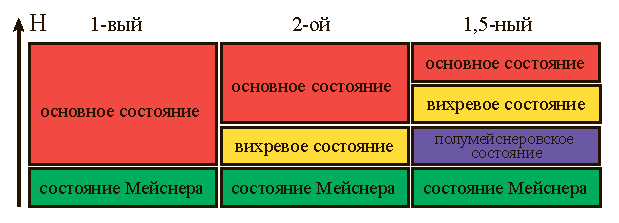
\includegraphics[width=.5\textwidth]{1-01}
  \caption{A comparison of the magnetic phase diagrams of
    clean bulk type-I,type-II and type-1.5 superconductors at
    zero temperature. The semi-Meissner state is a macroscopic
    phase separation into two-component Meissner state and vortex
    clusters where one of the density modes is suppressed by
    core overlaps}
  \label{fig:1}
\end{figure}

на невозможно параметризовать модель с точки зрения одного безразмерного 
параметра \( \kappa \). In the case where the condensates are not coupled by 
interband Josephson coupling but only by the vector potential these length 
scales arethe two independent coherence lengths (set by the inverse masses of 
the corresponding scalar density fields) and magnetic field penetration length 
(set by the inverse mass acquired by the gauge field). In contrast, in the 
case where the condensates are coupled by inter-band Josephson terms, one 
cannot distinguish independent coherence lengths attributed to different 
condensates. Nonetheless, in this case the density variations can also possess 
two fundamental length scales\cite{bib:2}, in contrast to single-component 
theories. We elaborate on this fact below. In \cite{bib:1,bib:2} vortex 
solutions in two-component theories were found which have non-monotonic 
vortex inter-action, with a long range attractive part determined by a 
dominant density-density interaction and a short range repulsive part produced 
by current-current and electro-magnetic interactions. An important 
circumstance which was demonstrated was that these vortices are 
thermodynamically stable in spite of the existence of the attractive tail in 
the interaction.

A non-monotonic intervortex interaction potential should result in the 
formation of vortex clusters in low magnetic field immersed into the 
vortexless areas, a state referred to in \cite{bib:1} as the "semi-Meissner 
state". Figure \ref{fig:1} shows the schematic phase diagram of a type-1.5 
superconductor.

If the vortices form clusters one cannot use the usual one-dimensional 
argument concerning the energy of superconductor-to-normal state boundary to 
classify the magnetic response of the system. First of all, the energy per 
vortex in such a case depends on whether a vortex is placed in a cluster or 
not: i.e. formation of a single isolated vortex might be energetically 
unfavorable, while formation of vortex clusters is favorable, because in a 
cluster where vortices are placed in a minimum of the interaction potential, 
the energy per flux quantum issmaller than that for an isolated vortex 
(thermodynamically the nonmonotonic two-vortex interaction potential predicts 
that the smallest energy per flux quantum will be in the case of a uniform 
lattice with spacing equal to the minimum of two-body intervortex potential).

Thus, besides the energy of a vortex in a cluster, there appears an additional 
energy characteristic associated with the boundary of a cluster. In other 
words, in this situation, to determine the magnetic response of a system it is 
not sufficient to study the one-dimensional boundary problem nor the 
single-vortex problem, in contrast to single component systems. Moreover, in a 
cluster the system tends to minimize the boundary energy of a cluster 
(similarly to type-I behavior), while breaking into a lattice of one-quantum 
vortices inside the cluster (similarly to type-II systems with negative 
interface energy). Thus, in an increased magnetic field the vortices form via 
a first order phase transition. A magnetic phase distinct from the vortex and 
Meissner states which then arises is a macroscopic phase separation into 
domains of two-component Meissner state and vortex clusters where one of the 
density modes is suppressed by core overlap. We summarize the basic properties 
of type-I, type-II and type-1.5 regimes in the table I.

Существование термодинамически устойчивых сверхпроводящих типа 1.5 в конечном 
счете, зависит от существования немонотонного межвихревого потенциала 
взаимодействия. It is an important question how generic this effect is. В этой 
работе мы в основном сосредоточены на многополосных реализациях 
многокомпонентной сверхпроводимости и исследованию эффекта межзонной 
джозефсоновской связи, связи смешанного градиента, и связь типа 
плотность-плотность на вихревых взаимодействиях в двухзонных сверхпроводниках. 
Покажем, что (i), когда эти соединения присутствуют, система по-прежнему может 
обладать три основными масштабными длинами, в отличие от двух пространственных 
в обычной однокомпонентной теории ГЛ; (ii) немонотонное взаимодействие 
возможно в широком диапазоне изменения параметров в этих моделях.

Структура данной работы состоит в следующем: В разделе II вводится модель. 
В разделе III мы представляем линейную теорию асимптотики вихревых полей в 
двухполосных сверхпроводниках с различной межзонной связью.

We begin section III by demonstrating that for a general form of the effective 
potential in a two-band (or more generally two-gap) Ginzburg-Landau free 
energy, the linear theory gives, under quite general conditions, two 
fundamental length scales of the variations of the densities. From the 
linearized theory we calculate the long-range intervortex interaction 
potentials using the two-component generalization of the point-vortex method 
\cite{bib:19} and show how the non-monotonic intervortex interaction potential 
arise from the interplay of two fundamental length scales of the superfluid 
density variations and the magnetic field penetration length. The central 
point of this part is how the fundamental length scales are defined in the 
presence of interband coupling as well as the occurrence of "mode mixing". 
Next we move to quantitatively study the effects of several kinds of 
intercomponent couplings which quite generically arise in two-component 
theories.

In section III (d) we demonstrate that that mixed gradient coupling can lead 
under certain conditions to an increase in the disparity of the characteristic 
scales of the density variations.

В разделе IV мы представляем большое численное исследование полной нелинейной 
задачи взаимодействия между парой вихрей.
